\section{Confocal Vertex Parametrization}

We describe two parametrizations for billiard 3-periodic vertices: (i) standard and (ii) Jacobi.

\subsection{Standard}
\label{sec:02-confocal-standard-param}

We call ``standard'' parametrization that where a first vertex $P_1(t)$ of the billiard 3-periodic is parametrized as $P_1(t)=[x_1,y_1]=[a\cos{t},b\sin{t}]$.

As derived in \cite{garcia2019-incenter}, $P_2=(x_2,y_2)/q_2$ and $P_3=(x_3,y_3)/q_3$ where:

 \begin{equation}
 \label{eq:02-p2}
 \aligned 
x_{2}=&-{b}^{4} \left(  \left(   a^2+{b}^{2}\right)\cos^{2}\alpha   -{a}^{2}  \right) x_1^{3}-2{a}^{6} \,\cos  \alpha  \sin   \alpha  \, y_1^{3}\\
&+{a}^{4} \left(  ({a
}^{2}-3\, {b}^{2}) \cos^{2} \alpha  +{b}^{2}
 \right) {x_1}\,y_1^{2}-2\,{a}^{4}{b}^{2} \cos \alpha  \,\sin  \alpha    x_1^{2}{y_1},
\\
y_{2}=& 2{b}^{6} \,\cos \alpha\sin \alpha\,   x_1^{3}-{
a}^{4}  \left(  \left(   a^2+{b}^{2}\right)\cos^{2}  \alpha  -{b}^{2}  \right)  y_1^{3}\\
&+  2\,{a}^{2} {b}^{4}\cos \alpha \sin
  \alpha \; {x_1} y_1^{2} +{b}^{4}\left(  ({b
 }^{2}-3\, {a}^{2}) \cos^{2} \alpha  +{a}^{2}
  \right) x_1^{2}{y_1}
\\
q_2=&{b}^{4} \left( a^2-(a^2-b^2)\cos^2  \alpha   \right)
x_1^{2}+{a}^{4} \left(  {b}^{2}+(a^2-b^2)\cos^2 \alpha  
 \right) y_1^{2}\\
 & - 2\, {a}^{2}{b}^{2} \left({a}^{2} -{b}^{2} \right)\cos \alpha\sin \alpha \; {x_1}\,{
y_1}.
\endaligned
%
\end{equation}

 \begin{equation} \label{eq:02-p3} \aligned 
x_{3}\; =& \; {b}^{4} \left( {a}^{2}- \left( {b}^{2}+{a}^{2} \right) 
 \cos^{2}\alpha\right)   x_1^{3}+2\, {a}^{6} 
 \cos \alpha\,\sin \alpha\, y_1^{3}\\
 &+{a}^{4} \left( 
  \cos^{2}  \alpha  \left( {a}^{2}-3\,{b}^{2}
 \right) +{b}^{2} \right) { x_1}\, y_1^{2}+2\,{a}^{4}{b}^{2} \cos  \alpha\sin \alpha\,   x_1^{2}{ y_1}
\\
y_{3} \;=&\; -2\, {b}^{6} \cos \alpha\sin \alpha\, x_1^{3}+
{a}^{4} \left( {b}^{2}- \left( {b}^{2}+{a}^{2} \right)   \cos^{2}  \alpha  \right)\,  y_1^{3}\\
& -2\,{a}^{2}  {b}^{4}\cos
 \alpha  \sin \alpha\,  x_1 y_1^{2}+
{b}^{4} \left( {a}^{2}+ \left( {b}^{2}-3\,{a}^{2} \right)  \left( \cos
 \alpha  \right) ^{2} \right) {{ x_1}}^{2}{ y_1},
\\
q_3 \;=& \; {b}^{4} \left( {a}^{2}- \left(a^2 -{b}^{2}  \right)   \cos^{2} \alpha   \right) x_1^{2}+{a}^{4} \left( {b}^{2}+ \left( a^2-{b}^{2}  \right)  \cos^{2} \alpha  \right)  y_1^{2}\\
&+2\,{a}^{2}{b}^{
2} \left( {a}^{2}-{b}^{2} \right) \cos \alpha \sin \alpha\, { x_1}\,{ y_1}.
\endaligned
%
\end{equation}
where:
\[\cos \alpha={\frac {a^2 b  \, \sqrt {-{a}^{2}-{b}^{2}+2\,\sqrt {{a}^{4}-{b}^{2}{c}^{2}}}}{{c}^{2}\sqrt {{a}^{4}-{c}^{2} x_1^{2}}}}=
\frac{  a^2 b^2 \, \sqrt {2\delta-{a}^{2}-{b}^{2}}} {c^2\sqrt{ a^4y_1^2 + b^4x_1^2}  } \]

Note that in \cref{sec:03-cap-vtx-param} we generalize the above to any concentric, axis-parallel pair.

\subsection{Jacobi's Universal Measure}
\label{sec:02-confocal-jacobi-param}

Under the standard parametrization, we can obtain the ``position'' $t$ of $P=[x,y]$ on an ellipse:

\[ t=\tan^{-1}{\frac{a y}{b x}}. \]

As shown in \cref{fig:02-jacobi-param}(top), when a first vertex $P_1(t)$ in the billiard 3-periodic is parametrized in the standard way, though its position is linear on the $t$ parameter, it will drive motions of the other two vertices $P_2(t)$ and $P_3(t)$ which are both distinct and non-linear. 

Fortunately, a uniform parametrization exists, which goes back to Jacobi, for all Poncelet families, based on the so-called ``universal measure'', which linearizes the Poncelet map, see \cite{koiller2021-spatial}. Specifically, vertices are obtained at fixed multiples of a constant $\Delta{u}$ in the argument of certain Jacobi elliptic functions. This parametrization, adapted to the elliptic billiard case, appears in \cite{stachel2021-billiards,stachel2021-billiards-param} and is reproduced below. First let's recall a few useful definitions. 

The  notation adopted below is as \cite{armitage-2006}. 

\begin{definition}
The incomplete elliptic integral of the first kind $K(\varphi,k)$ is given by:
\begin{equation}
K(\varphi,k)=\int_0^{\varphi}\frac{d\theta}{\sqrt{1-k^2 \sin^2\theta}}
\label{eqn:02-ellipticK}
\end{equation}
%\end{definition}

%\begin{definition}
The complete elliptic integral of the first kind $K(k)$ is simply $K(\pi/2,k)$.
\end{definition}

\begin{definition}
The elliptic sine $\text{sn}$, cosine $\text{cn}$, and delta-amplitude $\text{dn}$ are given by:
\begin{align*}
\text{sn}(u,k)&=\sin\varphi\\
\text{cn}(u,k)&=\cos\varphi\\
\text{dn}(u,k)&=\sqrt{1- k^2\sin^2\varphi}\\
\end{align*}
where $\varphi=\text{am}(u,k)$ is known as the amplitude, i.e., the upper-limit in the integral in \cref{eqn:02-ellipticK} such that $K(\varphi,k)=u$.
\end{definition}
A review of these functions appears in \cref{app:appD-jacobi-functions}.

\begin{remark}
Note to the reader: Mathematica (resp. Maple) expects $m=k^2$ (resp. $k$) as the second parameter to elliptic functions.

With this terminology the  Jacobi elliptic functions are defined    as follows:
\begin{align*}
K(\varphi,m)&=\int_0^{\varphi} \frac{dy}{\sqrt{1-m\sin^2y}}=u,\;\; \varphi=\text{am}(u,m)\\
%K(\varphi,k)=u\\ %
\sn(u,m)&=\sin\varphi,\; \cn(u,m)=\cos\varphi,\; dn(u,m)=\sqrt{1-m\sin^2\varphi}, \end{align*}

%As a note the reader, Maple accepts $k$ while Mathematica requires $m=k^2$ as the argument to elliptic functions.

%For example, in Maple we have: \[\sn(2,0.4)=\texttt{JacobiSN(2,.4)}=0.94569756\ldots\]
%and in Mathematica:

%\[ \sn(2,0.16)=\texttt{JacobiSN[2,.16]}=0.945698 \ldots \]
%and
%\[ \texttt{JacobiSN[2,.4]}=0.985090\ldots \]
\end{remark}

\begin{theorem}
A billiard orbit $P_i$ $(i=1,\ldots, N) $ of period $N$  with turning number $\tau$, where $\mathrm{gcd}(N,\tau) =1$,  is parametrized on $u$ with period $4K$ where:


\[ 
P_i=
%=\left[a\; \Jsn \left(u+\frac{4n\tau K}{N}, \frac{c}{a}\right), b\; \Jcn \left(u+\frac{4n\tau K}{N}, \frac{c}{a}\right)\right]\\
\left[-a\,\sn  \left(u+ i \Delta{u},  {m} \right) , b\,\cn  \left(u + i \Delta{u}, { m} \right)\right]
\]

where,
\[ m=k^2=\frac{a_c^2-b_c^2}{a_c^2},\;\;\Delta{u}=\frac{4\tau K}{N}\]
\[a= \sqrt{b^2+ a_c^2-b_c^2}, \;\; b=\frac{b_c}{\cn(\frac{\Delta{u}}{2}, m)}\]
\end{theorem}
\begin{proof} See \cite{stachel2021-billiards}.\end{proof}

A basic fact to obtain this parametrization is the following.

\begin{figure}
    \centering
    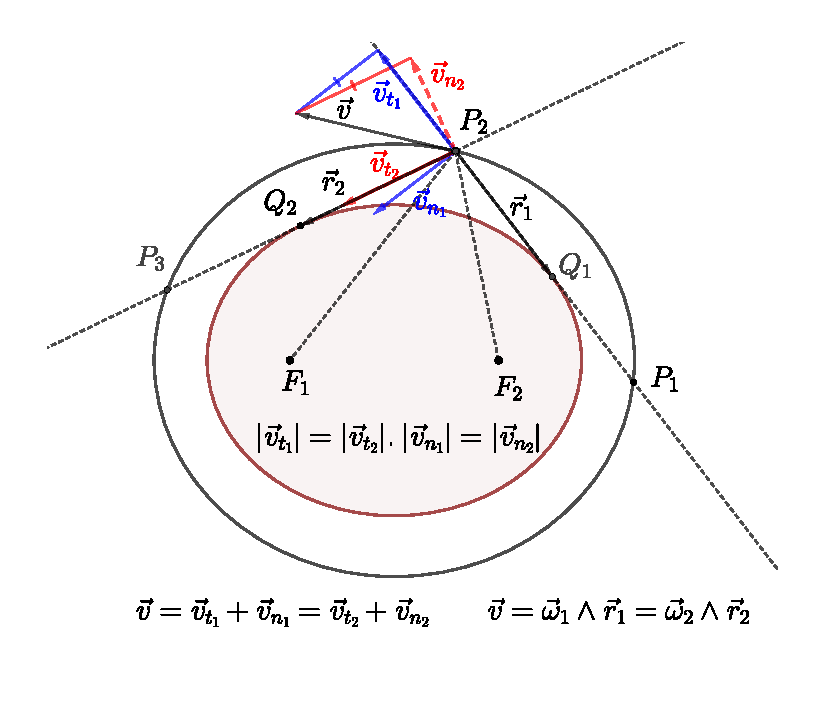
\includegraphics[width=\textwidth]{pics_02_040_param_jacobi.pdf}
    \caption{ Angular velocity $\vec v=\vec \omega\wedge \vec r$. } 
    \end{figure}
Referring to \cref{fig:02-velocidade-angular}:

\begin{proposition} 
Consider   segment of orbits $P_1P_2$ and $P_2P_3$  and contact points $Q_1$ and $Q_2$ with the caustic in an elliptic billiard. Let $\vec v$ the vector velocity of $P_2(t)$. Let $\vec r_1=Q_1-P_2$ and $\vec r_2=Q_2-P_2$. Then
\[ |\vec \omega_1|\;|\vec r_1|=|\vec \omega_2|\; |\vec r_2|\]
where $\vec v=\vec\omega_1\wedge r_1= \vec\omega_2\wedge \vec r_2$.

\label{fig:02-velocidade-angular}
\end{proposition}

\begin{proof} Let $\vec v=P_2'(t)$. From Graves's theorem, $|\vec r_1|+|\vec r_2|-\text{arc}(Q_1,Q_2)=\text{cte}$,  and therefore it follows that in decomposition of $\vec v=\vec v_{t_1}+\vec v_{n_1}=\vec v_{t_2}+\vec v_{n_2}$ we have that $|\vec v_{t_1}|=|\vec v_{t_2}|$ and  $|\vec v_{n_1}|=|\vec v_{n_2}|$. The result follows from the   definition of angular velocity. More details see \cite{stachel2021-billiards-param}.
\end{proof}
 
\textcolor{red}{ronaldo}
 
Since in this chapter we are considering billiard 3-periodics, so above $N=3$, and $\tau=1$. As shown in \cref{fig:02-jacobi-param}, under the Jacobi parametrization each of the 3 vertices of billiard 3-periodics follows the exact same curve, albeit with a 120-degree phase.

Recall the sum of cosines is constant for billiard 3-periodics. \cref{fig:02-jacobi-cos-param} shows how individual cosines follow either (i) 3-distinct curves, or (ii) the same exact curve (at different phases) if the parametrization is standard or Jacobi, respectively.

\begin{figure}
    \centering
    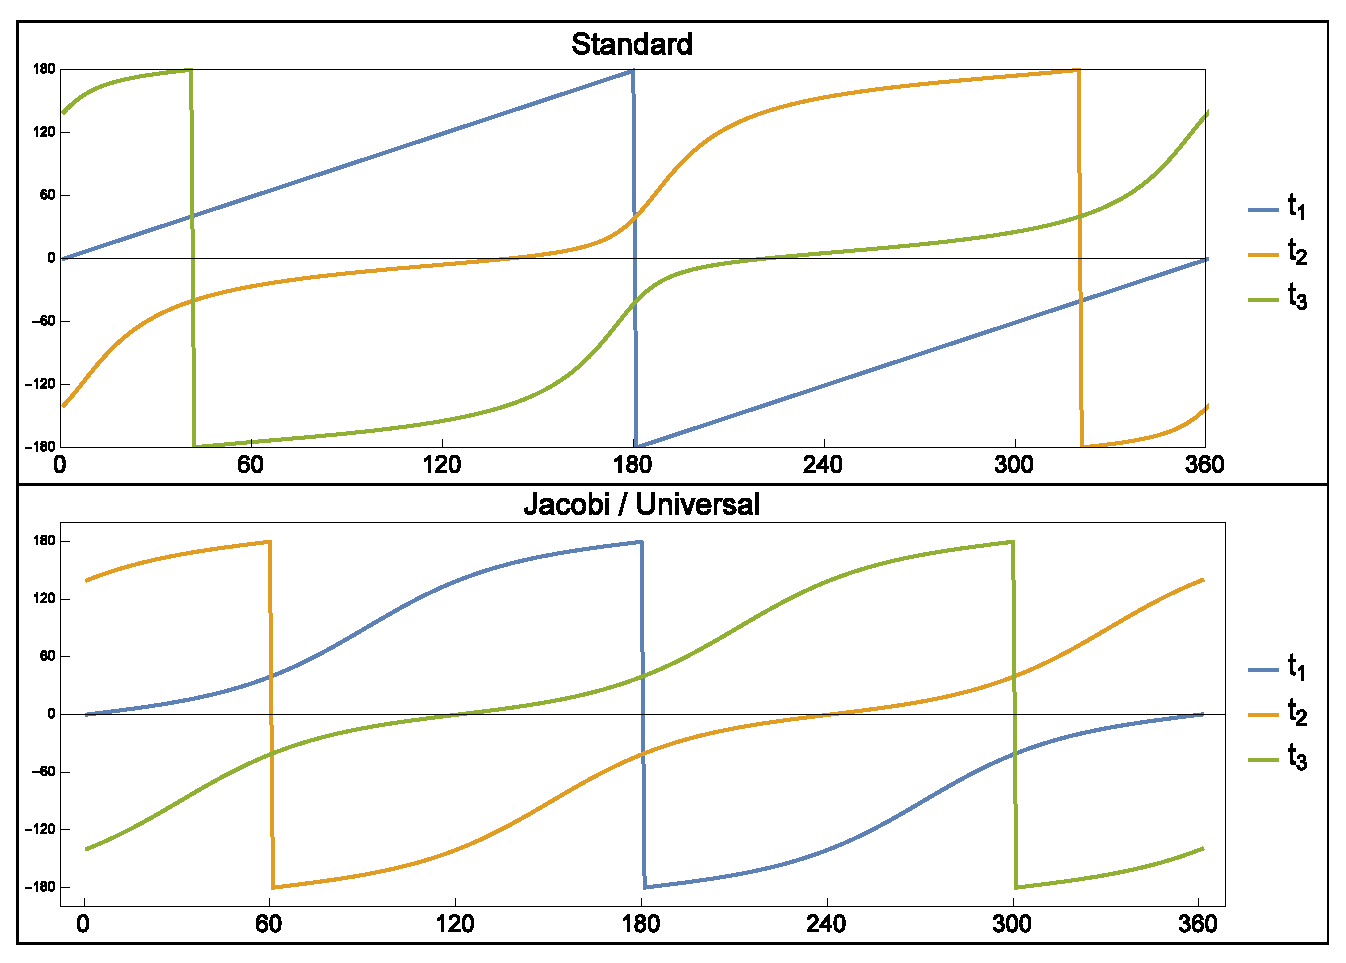
\includegraphics[width=\textwidth]{pics_02_050_parametrizations}
    \caption{The ``position'' $\theta_i$ (vertical axis) of a point on an ellipse with semi-axes $a,b$ vs the billiard 3-periodic parameter (horizontal axis). \textbf{Top:} vertex  under ``standard parametrization'', i.e., $P_1(t)=[a\cos{t},b\sin{t}]$. Notice while $P_1$'s position evolves linearly, those of $P_2$ and $P_3$ are different curves. \textbf{Bottom:} Said positions under Jacobi's parametrization. Notice the three positions are 120-degree delayed copies of one another.}. 
    \label{fig:02-jacobi-param}
\end{figure}

\begin{proof}
\textcolor{red}{ronaldo}
\end{proof}
\begin{figure}
    \centering
    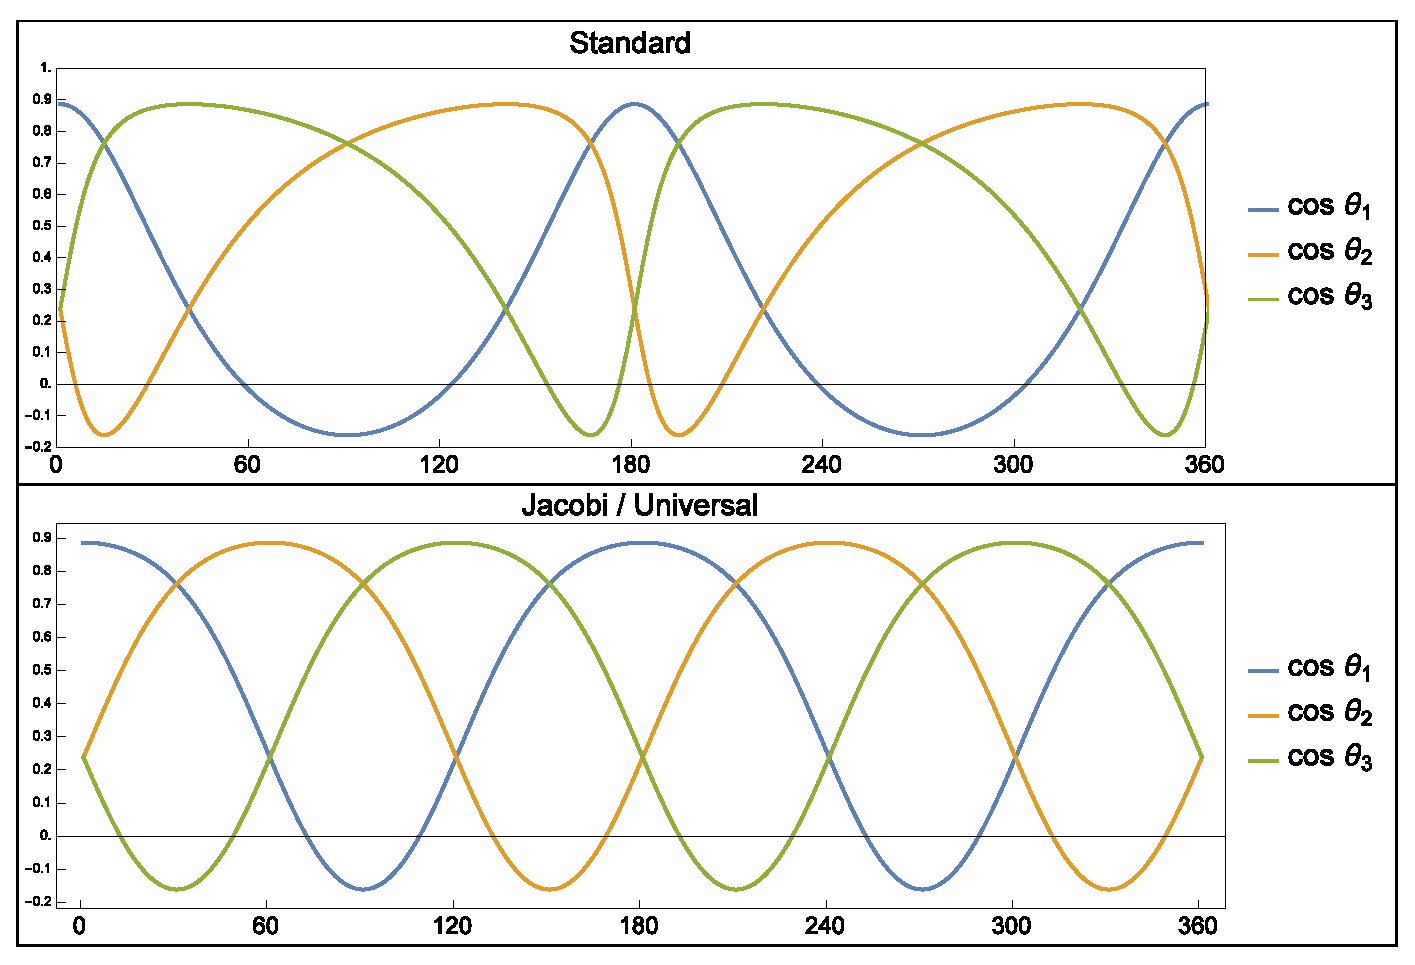
\includegraphics[width=\textwidth]{pics_02_060_cos_parametrizations}
    \caption{The cosines $\cos(theta_i)$ of billiard 3-periodic internal angles for the standard (top) and Jacobi parametrizations (bottom). While in the former case the three curves are distinct, in the latter case all cosines follow the same curve at different phases.}
    \label{fig:02-jacobi-cos-param}
\end{figure}
